% -*- TeX-PDF-mode: t ; ispell-dictionary: "french"; -*- 
\documentclass[a4paper]{article}

\usepackage[frenchb]{babel}
\usepackage{xunicode}
\usepackage{xltxtra}
\defaultfontfeatures{Mapping=tex-text}
\usepackage{fontspec}
\usepackage{xcolor,url,graphicx}
\usepackage{tikz}
\usetikzlibrary{positioning}
\usepackage[pdfauthor={Philippe Wang mail@philippewang.info},pdftitle={Moi et les macarons parisiens},pdfsubject={Gastronomie fran\,caise},pdfcreator={XeLaTeX}]{hyperref}
% sans serif
\def\SSSCfont{Fontin Sans Small Caps}
\def\SSfont{Fontin Sans}

% roman
\def\RMfont{Baskerville}
\def\RMfont{Fontin}

% roman small caps
\def\RMSCfont{Fontin SmallCaps}

% tt
\def\Monofont{Menlo}
%\def\Monofont{Andale Mono}
\def\Monofont{Monaco}

\setsansfont[SmallCapsFont={\SSSCfont}]{\SSfont} % choix final ?
\setromanfont[SmallCapsFont=\RMSCfont]{\RMfont}
\setmonofont[Scale=0.8]{\Monofont}


\title{Moi et les macarons parisiens}
\author{Philippe \sc Wang\\\href{mailto:mail@philippewang.info}{\sc\small Mail@PhilippeWang.info}}


\newcommand{\guillemets}[1]{«#1»}




\def\tab{
  \begin{tabular}{|r|r|r|r|}\hline
    ingrédient      & quantité & quantité & quantité  \\\hline
}
\def\graph{
  \begin{tikzpicture}
  }
\gdef\startx{0}
\def\ingredient#1#2{
  \draw [fill=#1] (\startx,0) rectangle +(0.2,#2/100);
  \expandafter\gdef\expandafter\startx\expandafter{\startx+0.3}
}

\newcommand\oeuf[3]{
  \expandafter\def\expandafter\tab\expandafter{\tab
    blanc d'oeuf & #1 & #2 & #3\\\hline
  }
  \expandafter\gdef\expandafter\graph\expandafter{\graph
    \ingredient{white}{#2}
  }
}
\newcommand\amande[3]{
  \expandafter\gdef\expandafter\tab\expandafter{\tab
    poudre d'amande & #1 & #2 & #3\\\hline
  }
  \expandafter\gdef\expandafter\graph\expandafter{\graph
    \ingredient{yellow}{#2}
  }
}
\definecolor{csglace}{rgb}{0.1,0.6,0.1}
\newcommand\sglace[3]{
  \expandafter\gdef\expandafter\tab\expandafter{\tab
    sucre glace & #1 & #2 & #3\\\hline
  }
  \expandafter\gdef\expandafter\graph\expandafter{\graph
    \ingredient{csglace}{#2}
  }
}
\definecolor{cspoudre}{rgb}{0.5,1,0.5}
\newcommand\spoudre[3]{
  \expandafter\gdef\expandafter\tab\expandafter{\tab
    sucre en poudre & #1 & #2 & #3\\\hline
  }
  \expandafter\gdef\expandafter\graph\expandafter{\graph
    \ingredient{cspoudre}{#2}
  }
}
\newcommand\eau[3]{
  \expandafter\gdef\expandafter\tab\expandafter{\tab
    eau & #1 & #2 & #3\\\hline
  }
  \expandafter\def\expandafter\graph\expandafter{\graph
    \ingredient{blue}{#2}
  }
}
\newcommand\stopingredients{
  \expandafter\def\expandafter\tab\expandafter{\tab
    \end{tabular}
  }
  \expandafter\def\expandafter\graph\expandafter{\graph
    \end{tikzpicture}
  }
  % \begin{tabular}{|l|l|}\hline
    \tab 
    % &
    \graph
    % \\\hline
    % \end{tabular}
}
\newcommand\resetingredients{
  \def\tab{
    \begin{tabular}{|r|r|r|r|}\hline
      ingrédient      & quantité & quantité & quantité  \\\hline
    }
  \def\graph{
      \begin{tikzpicture}
      }
  \gdef\startx{0}
}





\begin{document}
\maketitle
\begin{tikzpicture}[overlay,remember picture]
  \node at (5.5cm,7cm) {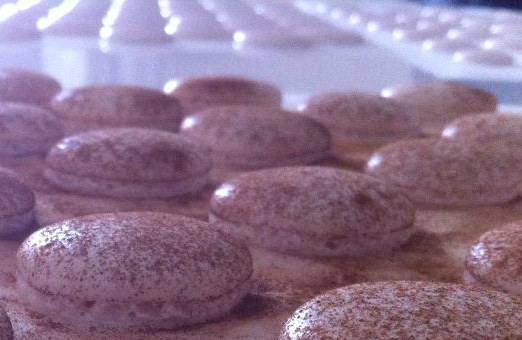
\includegraphics[height=5cm]{macarons}};
\end{tikzpicture}

%\section{Introduction}
Les macarons  parisiens sont  des pâtisseries à  la mode,  délicats en
apparence mais aussi délicats à  réaliser.  Quant aux goûts du macaron
parisien, ils  varient selon l'auteur  de l'assemblage des  parfums et
plus  particulièrement du  goût du  fourrage utilisé,  bien  sûr, mais
aussi de l'humeur de celui qui les déguste.  La texture, quant à elle,
varie selon la réussite des  coques de macarons, de leur conservation,
et de leur fourrage. %C'est ce mélange de textures et de saveurs qui


Ces macarons  sont connus pour  être des gâteaux colorés,  souvent aux
couleurs  vives qui  marquent  l'esprit. Leur  apparence  a une  forte
influence sur la  manière dont on les déguste:  c'est pour cela qu'ils
sont si  souvent colorés... avec des  colorants qui ne  donnent pas de
goût si ce n'est qu'ils influent l'esprit du gourmand et que cela a en
fait un impact non négligeable sur  le goût.  On aura bien compris que
si on  mange des macarons dans  le noir, les  colorants n'auront aucun
effet sur le  goût!  Cela dit, si les colorants sont  en fait du cacao
en poudre  ou du  paprika, bien  sûr qu'ils ont  une influence  sur le
goût.

Dans cet article, je propose une synthèse des différentes approches de
la  réalisation de  macarons  parisiens.   Je me  base  sur ma  propre
expérience de réalisation de macarons  ainsi que sur des livres et des
sites web.

\section{Précision du travail}

On dit  souvent qu'en pâtisserie,  on travaille au gramme  près (alors
qu'en cuisine c'est  plus souple).  Je ne suis  pas vraiment d'accord.
Il y  a de très nombreuses  pâtisseries qu'il n'est  pas nécessaire de
travailler au gramme près. Mais derrière ce dicton qui donne une image
de  discipline militaire, se  cache une  assez grande  complexité.  En
fait,  en pâtisserie, des  fois, on  a besoin  d'un travail  de grande
précision,  et il  faut alors  travailler au  gramme près  (et parfois
encore plus précisément). Alors  c'est plus simple d'appliquer tout le
temps la règle  du travail au gramme près, plutôt que  de faire du cas
par cas. 

Alors  pour  les  macarons  parisiens?   Si  on  regarde  un  peu  les
différentes  recettes qu'on  peut  trouver, tout  d'abord on  constate
qu'elles sont  très nombreuses, similaires mais  avec des différences,
que ce soit de technique ou de proportions, etc. On est vite perdu.

Les macarons sont réputés comme  étant difficiles à réussir. Pour moi,
cela vient principalement de  l'imprécision des recettes en général et
cette  sorte de  volonté  de  ne pas  vouloir  imposer une  discipline
stricte aux lecteurs et de laisser une grande part au hasard.


\subsection{Respect des proportions}

\textbf{La première imprécision vient de la quantité de blanc d'oeuf.}  

En général,  les recettes  indiquent une quantité  de blanc  d'oeuf en
terme   de   nombre   d'oeuf.   Par  exemple,   \guillemets{2   blancs
  d'oeuf}.  Ensuite, parfois  ils  indiquent qu'un  blanc d'oeuf  fait
environ 35g.  Quelques fois,  si on a  un peu  de chance, on  voit que
l'auteur met  une réserve  si jamais les  blancs d'oeuf font  un poids
différent.

À moins de travailler dans  une cuisine professionnelle avec des oeufs
en bidon (où les blancs et  les jaunes sont dans des bidons différents
bien sûr), on a peu de chances d'avoir des blancs d'oeuf qui font pile
poil 35g. Mais comme c'est une valeur moyenne, plus on utilise d'oeufs
et plus on a en moyenne des  blancs d'oeuf de 35g.  Par exemple, si je
casse un oeuf, je risque d'avoir  un blanc d'oeuf qui fait entre 25 et
45g. Si  je casse dix  oeufs, j'ai plutôt statistiquement  des grandes
chances d'avoir  entre 300 et 400g  de blanc d'oeuf (et  non pas entre
250g et  450g) et même que j'ai  de bonnes chances d'avoir  350g à 10g
près. Cela dit, on ne veut pas toujours utiliser une dizaine d'oeufs 
pour faire des macarons! (10 oeufs, à la louche ça doit être assez
pour faire 300 à 450 coques de macarons d'environ 3,5cm de diamètre)

La solution que je propose est simple: il faut se baser sur la
quantité de blanc d'oeuf car c'est l'ingrédient dont la quantité qu'on
va obtenir en cassant des oeufs est impossible à deviner avant de
casser les oeufs.  

\textbf{N.B. J'ai pu constater que souvent, les oeufs bio ont des jaunes plus gros.}

Cependant, ce n'est pas une obligation  de se baser sur la quantité de
blanc d'oeuf. L'important est de bien respecter les proportions.

Si vous voulez vous baser par exemple sur la quantité de poudre
d'amande, par exemple parce que vous n'en avez que 65g exactement,
c'est possible.  Avec 65g d'amande, si on fait le calcul d'après
\cite{masterchef:2011}, il faut 52g de blanc d'oeuf, ce qui fait
un énorme blanc d'oeuf  ou bien un peu moins de deux. Donc vous casserez
probablement deux oeufs et vous aurez un peu trop de blanc, que vous
pourrez utiliser dans une omelette par exemple.


\section{Deux techniques de réalisation de l'appareil à coques}

\subsection{La technique de la meringue italienne:
  sucre cuit sur les blancs d'oeuf}

\subsubsection{Proportions d'après \cite{masterchef:2011}}

% \begin{tabular}{|r|r|r|r|r|}\hline
%   ingrédient & quantité & quantité & quantité & quantité\\\hline
%   blanc d'oeuf & 1 & 100 & 80 & 0,8 \\\hline
%   poudre d'amande & 1,25 & 125 & 100 & 1 \\\hline
%   sucre blanc & 1,25 & 125 & 100 & 1 \\\hline
%   sucre glace & 1,25 & 125 & 100 & 1 \\\hline
%   eau & 0,31 & 31 & 25 & 0,25 \\\hline
% \end{tabular}

\oeuf   {100}{100}{ 80}
\amande {125}{125}{100}
\sglace {125}{125}{100}
\spoudre{125}{125}{100}
\eau    { 31}{ 31}{ 25}

\stopingredients
\resetingredients



Les quantités sont en grammes ou toute autre unité de mesure de masse.
Ces proportions \textbf{ne} peuvent \textbf{pas} s'appliquer à une mesure volumique.

\emph{C'est cette proportion que j'utilise le plus souvent.}

\subsubsection{Étapes de réalisation}

\paragraph{Tâche 1.}
Séparer en deux quantités égales le blanc d'oeuf.

~

Les tâches 2 et 3 peuvent être faites en même temps.

\paragraph{Tâche 2.}
\begin{enumerate}
\item  Battre (très)  lentement la  moitié du  blancs d'oeuf  pendant 30
  secondes, pour dérouler les  protéines, puis battre à grande vitesse
  pour qu'ils montent.   (Si on bat à grande vitesse  dès le début, on
  risque  de   casser  les  protéines   et  la  montée   devient  plus
  incertaine.)
\item Mettre le sucre blanc au centre d'une casserole et ajouter l'eau
  sur les côtés sans faire de projection. Attendre un peu que ça
  fonde, puis cuire jusqu'à 118°C (si ça caramélise, c'est que ça a
  largement dépassé 118°C et que vous n'avez plus qu'à recommencer en
  faisant plus attention)
\item Quand le sucre fait 118°C, le  verser en au moins 3 fois sur les
  blancs montés  (le premier versement  ne doit pas dépasser  le tiers
  pour  ne pas  trop chauffer  localement les  blancs), et  fouetter à
  vitesse maximale pendant une  minute. Vous pouvez ensuite réduire la
  vitesse (pour que  ça fasse moins de bruit et  que le moteur chauffe
  moins) jusqu'à ce que la meringue italienne ait une texture crémeuse
  (elle devrait alors faire maximum 45°C).
  \emph{Attention à ne pas verser beaucoup trop lentement le sucre: il durcit
    en refroidissant! Et attention à ne pas verser le sucre sur le fouet car
    il refroidirait très rapidement et se figerait, ce qui diminuerait 
    la quantité de sucre incorporé dans la meringue, ce qui fausserait
    les quantités, donc compromettrait la recette.}
\end{enumerate}

\paragraph{Tâche 3.}

\begin{enumerate}
\item passer au tamis le sucre glace et la poudre d'amande.
  Si la poudre d'amande n'est pas assez fine, la passer au mixeur avec 
  un peu de sucre glace (ou la totalité), selon la capacité de votre mixeur.
  Vous aurez peut-être à faire cela en plusieurs fois.
  Si votre poudre d'amande fait une masse pendant le passage au mixeur, 
  vous avez trois solutions:
  \begin{enumerate}
  \item soit vous faîtes confiance au mixeur et vous utilisez
    directement cette masse sans la passer au tamis
  \item soit vous passez quand même le mélange au tamis (c'est juste
    un peu plus difficile)
  \item  soit  avant le  passage  au  mixeur,  vous passez  la  poudre
    d'amande au four pour la sécher  un peu (sans la griller), dans ce
    cas, faîtes attention au poids de l'amande qui a peut-être pas mal
    diminué.
  \end{enumerate}
\item Si vous n'avez pas déjà mélangé le sucre glace et la poudre d'amande,
  mélangez les avec un fouet pour éviter de former des masses.
\item Ajoutez la  moitié des blancs d'oeuf et  mélangez pour former un
  appareil homogène.
\end{enumerate}

Avoir une poudre d'amande assez fine est primordial, car avoir une poudre
grossière revient à diminuer la surface de contact entre la matière 
sèche (la poudre d'amande)  et la matière liquide (le blanc d'œuf).


\emph{Astuce: si vous avez du mal à obtenir deux parts égales ou si
  vous avez trop peu de blanc d'oeuf pour arriver à les monter en
  neige, montez tout en neige, puis séparez à ce moment en deux parts
  égales, l'une pour continuer la tâche 2 (donc l'ajout de sucre cuit)
  et l'autre pour la tâche 3. }


\paragraph{Tâche 4. Le macaronage.}
Il ne reste plus qu'à ajouter en  3 ou 4 fois la meringue italienne au
mélange à base d'amande, et à mélanger (macaroner) jusqu'à l'obtention
d'une pâte lisse, brillante et un peu coulante.

Il ne faut pas que le macaronage dure trop longtemps car ça liquéfie
la pâte, mais un macaronage trop court donne une pâte trop peu homogène.

Si la pâte  est trop liquide, il faudra  attendre plus longtemps avant
la cuisson pour qu'elle sèche. (La cause la plus fréquente de la pâte
trop liquide, hormis le non respect évident des proportions de la recette,
vient d'une poudre d'amande trop grossière plutôt que d'un macaronage
raté.)


\subsection{La technique de la meringue française: sucre en poudre sur les blanc d'oeuf}


\subsubsection{Proportions d'après \cite{hermé:desserts}}

Pierre Hermé indique 7 blancs d'oeuf dans sa recette
\cite{hermé:desserts}, ce qui n'est pas très précis. Il indique dans
le même livre qu'un blanc d'oeuf fait en moyenne 34g. Partant sur
cette base, 7 blancs d'oeuf font 238g et les proportions sont alors
les suivantes:\\


% \begin{tabular}{|r|r|r|r|}\hline
%   ingrédient      & quantité & quantité & quantité  \\\hline
%   blanc d'oeuf    & 238      & 100      & 85        \\\hline
%   poudre d'amande & 280      & 118      & 100       \\\hline
%   sucre glace     & 480      & 202      & 171       \\\hline
% \end{tabular}


\oeuf   {238}{100}{ 85}
\amande {280}{118}{100}
\sglace {480}{202}{171}
\spoudre{  0}{  0}{  0}
\eau    {  0}{  0}{  0}

\stopingredients
\resetingredients



\emph{Remarque. Pour sa recette de base, avec 480g de sucre glace,
  Pierre Hermé ajoute jusqu'à 9 gouttes de colorant alimentaire ou 40g
  de cacao sans changer la quantité des autres ingrédients.}

% Les quantités sont en grammes ou toute autre unité de mesure de masse.
% Ces proportions \textbf{ne} peuvent \textbf{pas} s'appliquer à une
% mesure volumique.


\subsubsection{Proportions d'après \cite{cuisine-facile.com:macarons}}

% \begin{tabular}{|r|r|r|r|}\hline
%   ingrédient      & quantité & quantité & quantité  \\\hline
%   blanc d'oeuf    & 35      & 1         & 0,87        \\\hline
%   poudre d'amande & 40      & 1,14      & 1       \\\hline
%   sucre glace     & 75      & 1,88      & 1,87       \\\hline
%   sucre blanc     & 7       & 0,2       & 0,17       \\\hline
% \end{tabular}


\oeuf   { 35}{100}{ 87}
\amande { 40}{114}{100}
\sglace { 75}{188}{187}
\spoudre{  7}{ 20}{ 17}
\eau    {  0}{  0}{  0}

\stopingredients
\resetingredients

\subsubsection{Proportions d'après \cite{recettemacaron.eu:macarons}}

% \begin{tabular}{|r|r|r|r|}\hline
%   ingrédient      & quantité & quantité & quantité \\\hline
%   blanc d'oeuf    & 100      & 1        & 0,8      \\\hline
%   poudre d'amande & 125      & 1,25     & 1        \\\hline
%   sucre glace     & 200      & 2        & 1,6      \\\hline
%   sucre blanc     & 30       & 0,3      & 0,24     \\\hline
% \end{tabular}

\oeuf   {100}{100}{ 80}
\amande {125}{125}{100}
\sglace {200}{200}{160}
\spoudre{ 30}{ 30}{ 24}
\eau    {  0}{  0}{  0}

\stopingredients
\resetingredients


\subsubsection{Proportions d'après \cite{marmiton.org:macarons}}

% \begin{tabular}{|r|r|r|r|}\hline
%   ingrédient      & quantité & quantité & quantité \\\hline
%   blanc d'oeuf    & 35       & 1        & 0,83     \\\hline
%   poudre d'amande & 42       & 1,2      & 1        \\\hline
%   sucre glace     & 74       & 2,11     & 1,76     \\\hline
%   sucre blanc     & 10       & 0,29     & 0,24     \\\hline
% \end{tabular}

\oeuf   { 35}{100}{ 83}
\amande { 42}{120}{100}
\sglace { 74}{211}{176}
\spoudre{ 10}{ 29}{ 24}
\eau    {  0}{  0}{  0}

\stopingredients
\resetingredients




\subsubsection{Étapes de réalisation}

\paragraph{Tâche 1.}
Tamiser ensemble le  sucre glace et la poudre  d'amande.

\paragraph{Tâche 2.}
Monter les blancs en neige ferme. Si la recette utilise du sucre en poudre,
l'incorporer au blanc quand ça commence à bien mousser pour faire un appareil
à meringue française.

\paragraph{Tâche 3.}
Verser très rapidement le mélange (sucre glace + poudre d'amande) en pluie  sur les blancs en neige (ou l'appareil à meringue française).
Et macaroner.







\section{Formation, croutâge et cuisson des macarons}

\subsection{Cuisson des macarons}

\subsubsection{La double plaque de cuisson}
Pourquoi utiliser  plusieurs plaques de  cuisson?  

Il y a deux étapes pour  obtenir une belle surface lisse non craquelée
sur  le  macaron. La  première  est  le  croûtage, c'est  l'étape  qui
consiste à sécher le dessus du macaron afin qu'il se forme une croûte.
Si la croûte est assez solide,  elle ne se craquellera pas. Mais c'est
la seconde étape qui fixe  la croûte, c'est-à-dire le passage au four,
donc la  cuisson. Cette étape doit  se passer avant que  le macaron ne
commence à gonfler, car dans le cas contraire, la coque sera fissurée.
Quand le  macaron commence  à gonfler, il  se forme une  collerette en
dessous.  Pour qu'elle  se forme,  il  faut que  la poussée  due à  la
cuisson se  fasse bien. Et  au final, pour  que le macaron  se décolle
bien, il faut que le bas du macaron soit bien cuit.

La double plaque permet de ralentir  la cuisson du bas du macaron (qui
est en  contact avec la  plaque).  Cela permet  au haut du  macaron de
cuire en premier.  

La double plaque va accumuler de la chaleur et la diffusera de manière
uniforme si elle  a une bonne conduction de  la chaleur.  Deux plaques
mises l'une sur  l'autre, bien lourdes, ne se  déformeront pas pendant
la cuisson: c'est pour cela qu'on utilise de préférence des plaques en
acier,  puisque c'est  lourd et  que ça  diffuse très  efficacement la
chaleur.   L'aluminium a  tendance  à se  déformer  beaucoup plus  que
l'acier. Il  faut bien sûr  des plaques qui s'enchevêtrent  bien l'une
sur l'autre pour  avoir un maximum de surface  de contact, sinon c'est
comme si  on n'avait  qu'une seule plaque  (l'air est un  très mauvais
conducteur de chaleur).

Certains utilisent 3 ou 4 plaques plutôt que seulement 2.

La pierre  de cuisson (pour  le pain et  les pizzas) est  un excellent
accumulateur  de chaleur,  mais la  chaleur n'est  pas du  tout rendue
uniformément  à cause  de  la  lenteur de  diffusion  (par rapport  au
métal). Si on cuit des macarons dessus, les macarons se déformeront un
peu n'importe comment pendant la cuisson.

\paragraph{Accumulation de chaleur et diffusion uniforme de la chaleur}
La cuisson des macarons est une  étape simple à réaliser si on dispose
du matériel nécessaire et qu'on  apprend à connaître son four. Mais ce
n'est pas tout, car elle dépend  également de la couleur des coques de
macaron.

\paragraph{Notes diverses}

\subparagraph{Douilles et poches à douilles} Pour les débutants, je
conseillerais des poches à douilles jetables sans douille mais juste
avec l'embout découpé.  Si on veut être plus écologique, les poches à
douilles réutilisables sont très bien mais il faut alors trouver la
bonne taille de douille.  L'important est bien sûr de prendre une
douille ni trop petite (ça risquerait de liquéfier la pâte) ni trop
grosse (ça risquerait de faire des grosses flaques).

\subparagraph{Poids des œufs}
\begin{itemize}
\item Les petits œufs (S) pèsent moins de 53 grammes.
\item Le poids des œufs moyens (M) est compris entre 53 et 63 g.
\item Le poids des gros œufs (L) est compris entre 63 et 73 g.
\item Les très gros œufs (XL) pèsent plus de 73 g.
\end{itemize}

\bibliographystyle{plain-fr}
\bibliography{references}
\end{document}
